\chapter{Architektur}
\label{Architektur}

\section{Design/Architektur}
Um eine Schnittstelle zwischen der Datenbankanwendung und dem Nutzer zu schaffen, existieren zwei verschiedene Anwendungen. Die Clientanwendung und die Datenbankanwendung basierend auf einer Rest-Api stellen unterschiedliche Komponenten in dieser Arbeit dar.

\subsection{Ziele der Architektur}

Für die Planung des Projekts stellen sich viele Fragen. Welches Framework soll für die Rest-API genutzt werden? Wie interagiert die Datenbank mit der Rest-API und welchen Output soll diese überhaupt produzieren?
Das Hauptziel der Anwendung ist die Antwort auf eine Datenbankanfrage in einer Index basierten Form, damit über RDMA auf den virtuellen Speicher zugegriffen werden kann,welcher die nötigen Daten bereitstellt.
Auf die Technologie Remote Direct Memory Access wird in dieser Arbeit jedoch nicht eingegangen. Es wird lediglich eine Basis für die Kommunikation und Nutzung einer Indexbasierten Datenbank geschaffen.
\\
Da die Frameworks Apache Arrow und Gandiva eine Java Schnittstelle bereitstellen wird in dieser Arbeit Java 8 benutzt. 
Aufgrund dieser Entscheidung bietet sich auch das Spring Framework für die Kommunikationsschnittstelle in Form einer REST-Api an.
Ziel ist es mithilfe von Apache Arrow einen schnellen Datenlayer bereitzustellen und mithilfe von Gandiva diese Daten zu filtern und zu prozessieren.

Durch die Technologie des Non-Volatile-Rams und der Maximierung der Kapazität des Speichers in Form von NVRam,ist die Idee große Datenmengen in den Hauptspeicher mithilfe von Apache Arrow zu legen und diese dann auszuwerten und Indexbasiert als Antwort an den Client zu liefern.

\subsection{Randbedingungen}
Aufgrund der hohen Kosten von NVRam ist es in dieser Arbeit nicht möglich sehr große Datensätze mit der Anwendung zu testen. Daher wird hier der normale gebräuchlicher Hauptspeicher getestet.

\subsubsection{Technische Randbedingungen}
Für das Framework Gandiva gibt es eine Java-Api welche eine JNI-Bridge benutzt und unter der Haube mit dem eigentlichen Gandiva C++ Code kommunziert.
Um Gandiva nutzen zu können ist ein Linux Betriebssystem oder ein MacOS Betriebssystem notwendig. Für den neuen M1-Chip ist bis jetzt kein Support angeboten.
Das Apache Arrow Framework enthält ebenfalls eine Java-Api und lässt sich somit als Build-Artefakt aus dem Maven-Central-Repository herunterladen.


\subsection{Technologie-Stack Datenbankanwendung}

Grundsätzlich besteht die Datenbankanwendung aus drei verschiedenen Technologie Layern, welche miteinander intern von unten nach oben und zurück kommunizieren und lässt sich somit einer Schichtenarchitektur zuordnen. 


\begin{figure}[h]
  \centering
  \begin{subfigure}[b]{1.0\textwidth}
    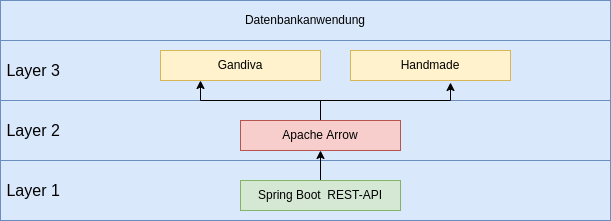
\includegraphics[width=1.0\linewidth]{img/layerarch}
  \end{subfigure}
  \caption{Technologie-Stack der DB-Anwendung}
  \label{graf_1}
\end{figure}

Im ersten Layer in \ref{graf_1} befindet sich das Spring-Boot Framework.
Dieses ist nötig um die Schnittstelle zwischen Client und Datenbankanwendung in Form einer Rest-Api sicher zu stellen. 
Über diese Rest-Api kann ein SQL-Dump mit verschiedensten Daten initialisiert werden, sowie Daten mithilfe von SQL-Queries abgefragt werden.

Die Anfragen werden dann mithilfe des Frameworks Arrow in Layer Zwei weiterverarbeitet. Dieser Layer Zwei kümmert sich um die Verwaltung der Daten im Speicher und ist das Herz der Datenbankanwendung. Über Arrow lassen sich die Daten in einem Spalten-Format im Hauptspeicher ablegen und aufrufen.

Im dritten Layer in \ref{graf_1} findet man das Framework Gandiva vor. 
Gandiva wird zum Filtern und zum Projizieren von den im Arrow-Format abgelegten Daten benutzt. Für den Fall das eine SQL-Query nicht mithilfe von Gandiva ausgewertet werden kann, kann hier eine Handmade-Implementierung genutzt werden.

\subsection{Einschränkungen der Datenbankanwendung}

Die Datenbankanwendung muss in der Lage sein SQL-Statements entgegen nehmen zu können. Da ein zu großer Aufwand besteht jede Art eines SQL-Statements abzudecken, wird in dieser Thesis der Umfang eingeschränkt. Jedoch wird im Abschnitt \ref{Erweiterungen} beschrieben wie man relativ einfach verschiedene Funktionen erweitern kann, da ein modulares Prinzip in der Entwicklung der Anwendung verwendet wird.

\subsubsection{Features der SQL-Statements}

\begin{itemize}
\item Der Table wird momentan im Statement nicht beachtet, da nur ein Table unterstützt wird 
 \item Es kann mithilfe eines Select-Statements auf einzelne, mehrere oder alle Spalten zugegriffen werden
 \item Falls ein Where-Statement benutzt wird, kann dieses nur auf eine einzelne Spalte angewendet werden
 \item Where-Statements werden momentan nur mit den Operatoren kleiner,größer und gleich unterstützt
 \item Es werden nur Abfragen unterstützt, welche Daten anfordern. Die Datenbank kann nicht mithilfe von Inserts bzw. Updates manipuliert werden.
\end{itemize}




\subsection{Technologie-Stack Clientanwendung}

Die Client-Anwendung basiert ebenfalls auf dem Spring-Boot Framework. Hier wird jedoch das Spring Shell Paket benutzt um eine interaktive Shell bereitstellen zu können.

Über die interaktive Shell kann eine Datenbank aus einem SQL-Dump initiliasiert werden oder einfache SQL-Queries versendet werden. Ebenfalls ist es möglich bestimmte Informationen über die Datenbank anzufragen.
Ziel der Datenbankanfragen ist es die nötigen Daten in einer Index-basierten Form zurückzuliefern, um später dann mithilfe von RDMA über die ebenfalls mitgelieferten Speicheradressen die Daten abfragen zu können.



